%\documentclass[a4paper]{article}
%\usepackage[utf8]{inputenc}
%\usepackage[spanish, es-tabla]{babel}
%
%\usepackage{amsmath}
%\usepackage{amsfonts}
%\usepackage{amssymb}
%
%\usepackage{booktabs}
%\usepackage[margin=0.8in]{geometry}
%\usepackage{float}
%\usepackage{graphicx}
%\usepackage{subcaption}
%\captionsetup{compatibility=false}
%
%\usepackage{multirow}
%\setlength{\doublerulesep}{\arrayrulewidth}
%
%\usepackage{array}
%\newcolumntype{C}[1]{>{\centering\let\newline\\\arraybackslash\hspace{0pt}}m{#1}}
%\newcommand\underrel[2]{\mathrel{\mathop{#2}\limits_{#1}}}
%\usepackage[american]{circuitikz}
%
%
%
%\usepackage{fancyhdr}
%
%\usepackage{units} 
%
%\pagestyle{fancy}
%\fancyhf{}
%\lhead{22.01 TC}
%\rhead{Mechoulam, Lambertucci, Rodriguez, Londero, Galdeman}
%\rfoot{Página \thepage}
\documentclass[a4paper]{article}
\usepackage[utf8]{inputenc}
\usepackage[spanish, es-tabla, es-noshorthands]{babel}
\usepackage[table,xcdraw]{xcolor}
\usepackage[a4paper, footnotesep = 1cm, width=20cm, top=2.5cm, height=25cm, textwidth=18cm, textheight=25cm]{geometry}
%\geometry{showframe}

\usepackage{tikz}
\usepackage{amsmath}
\usepackage{amsfonts}
\usepackage{amssymb}
\usepackage{float}
\usepackage{graphicx}
\usepackage{caption}
\usepackage{subcaption}
\usepackage{multicol}
\usepackage{multirow}
\setlength{\doublerulesep}{\arrayrulewidth}
\usepackage{booktabs}

\usepackage{hyperref}
\hypersetup{
    colorlinks=true,
    linkcolor=blue,
    filecolor=magenta,      
    urlcolor=blue,
    citecolor=blue,    
}

\newcommand{\quotes}[1]{``#1''}
\usepackage{array}
\newcolumntype{C}[1]{>{\centering\let\newline\\\arraybackslash\hspace{0pt}}m{#1}}
\usepackage[american]{circuitikz}
\usetikzlibrary{calc}
\usepackage{fancyhdr}
\usepackage{units} 

\graphicspath{{../Ejercicio-1/}{../Ejercicio-2/}{../Ejercicio-3/}{../Ejercicio-4/}}

\pagestyle{fancy}
\fancyhf{}
\lhead{22.01 Teoría de Circuitos}
\rhead{Mechoulam, Lambertucci, Rodriguez Turco, Londero, Galdeman}
\rfoot{\centering \thepage}

\begin{document}

\tableofcontents
\break
\section{auxiliar}

\subsection{Introducción Teórica}

\subsubsection{Filtros Activos con GIC}

Los inductores suelen ser los componentes electrónicos menos ideales a la hora de querer realizar un filtro. Esto se debe a varias razones: su tamaño en frecuencias bajas y por ende su peso, su resistencia interna grande en comparación a los capacitores, su dificultad a la hora del armado y más. Con el surgimiento del concepto de la realimentación en los circuitos electrónicos, se pudo mediante el uso de amplificadores operacionales, obtener cualquier tipo de respuesta en los filtros. Además, como los operacionales son dispositivos activos, estos pueden proveer al circuito la energía que es disipada por los resistores y aún más por medio de la alimentación que estos dispositivos requieren.

Sin embargo, varias limitaciones surgen por el uso de operacionales. La más importante suele ser la dependencia de la ganancia a lazo abierto con la frecuencia y su inconveniente respuesta a altas frecuencias. Esto suele ocasionar que los filtros activos tengan un rango de correcta operación por debajo de hasta los $100Mhz$. Afortunadamente cuanto mayor la frecuencia menores son las dificultades presentadas por el uso de inductores y esto hace que para este rango de frecuencias el inductor vuelva a ser una buena opción a la hora de implementar filtros.

Varias implementaciones de filtros activos han sido utilizadas históricamente, siendo una de estas el método de la síntesis directa. Este método se basa en utilizar distintos convertidores de impedancia como giradores o GICs. Este informe se centra, en el análisis e implementación de filtros utilizando el método de síntesis directa, entre otras cosas, comenzando con una breve explicación del funcionamiento de un GIC.

\subsubsection{Convertidor Generalizado de Impedancia o GIC}
Los convertidores generalizados de impedancia o GICs son circuitos activos diseñados para simular impedancias que cambian con la frecuencia. Se puede observar en la Figura (\ref{fig:gic}) una implementación de un GIC.

\begin{figure} [H]
	\centering
	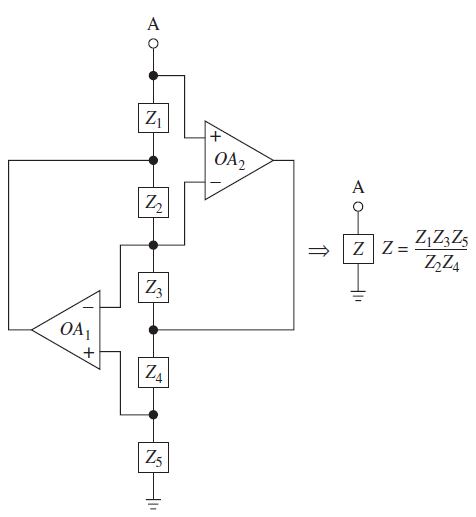
\includegraphics[width=0.6\textwidth]{Imagenes/gic.PNG}
	\caption{Convertidor generalizado de impedancia puesto a tierra[1].}
	\label{fig:gic}
\end{figure}

Estos circuitos están compuestos solamente por resistores, capacitores y amplificadores operacionales, por lo que sobresalen en su uso como emuladores de inductores o capacitores de gran capacidad.

\begin{figure}[H]
	\centering
	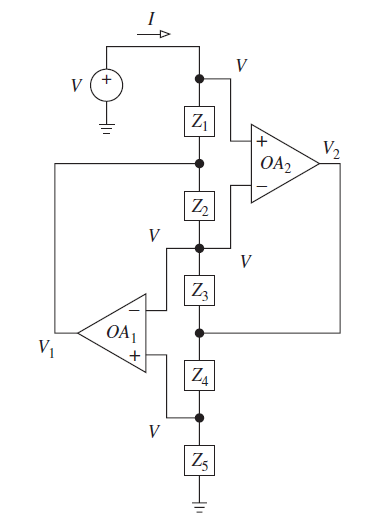
\includegraphics[width=0.5\textwidth]{Imagenes/gic_zin.PNG}
	\caption{Obtención de la impedancia de entrada del convertidor generalizado de impedancia puesto a tierra[2].}
	\label{fig:gic_zin}
\end{figure}

Para obtener la impedancia de entrada del GIC basta solamente calcular la corriente de entrada y utilizar la ley de nodos de Kirchhoff en los nodos de potencial V.

\begin{equation}
\frac{V-V_1}{Z_1}=I
\label{gic_zin_1}
\end{equation}

\begin{equation}
\frac{V_1-V}{Z_2} = \frac{V-V_2}{Z_3}
\label{gic_zin_2}
\end{equation}

\begin{equation}
\frac{V_2-V}{Z_4} = \frac{V}{Z_5}
\label{gic_zin_3}
\end{equation}

Utilizando (\ref{gic_zin_1}), (\ref{gic_zin_2}) y (\ref{gic_zin_3}) se llega finalmente a

\begin{equation}
Z_{in} = \frac{Z_1 Z_3 Z_5}{Z_2 Z_4}
\label{grounded_gic_zin}
\end{equation}

Esto demuestra que un GIC se puede utilizar para emular la impedancia que se desee, eligiendo convenientemente las impedancias $Z_1, \ Z_2, \ Z_3, \ Z_4 \ y \ Z_5$ dentro de las limitaciones que este posee.

\begin{figure}[H]
	\centering
	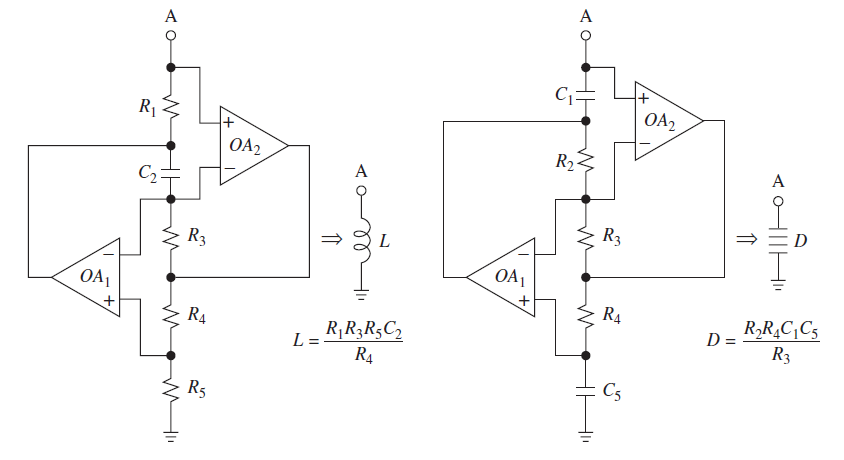
\includegraphics[width=1\textwidth]{Imagenes/gic_ind_fndr.PNG}
	\caption{Utilización de GICs para emular una inductancia a la izquierda y realizar un FNDR o elemento D a la derecha[3].}
	\label{fig:gic_ind_fndr}
\end{figure}

Como se puede observar en la Figura (\ref{fig:gic_ind_fndr}), dos implementaciones muy utilizadas de los GICs puestos a tierra son la de un inductor o un FNDR. Sin embargo, estas implementaciones poseen varias limitaciones a la hora de realizar el diseño de un filtro ya que por la naturaleza interna de los amplificadores operacionales, se debe tener en cuenta que debe haber un camino para la continua que pueda ser utilizada para polarizar correctamente los transistores en el interior de los operacionales. En el siguiente circuito se analizará e implementará un filtro activo con un GIC que no está no puesto a tierra.


\subsection{Análisis del Circuito}

En una primera instancia, se puede observar en la Figura (\ref{fig:circ_redibujado}) como el circuito a analizar consiste de un filtro de primer orden compuesto por un convertidor generalizado de impedancia cuya salida se encuentra realimentada a la entrada. Si bien la elección de las impedancias del GIC sugieren que este se comporta como un inductor y que el filtro será de segundo orden, la realimentación por la resistencia $R_8$ al potencial de entrada exige un análisis detallado de la función transferencia del circuito. Este será el primer paso a tomar en el análisis del filtro.

\subsubsection{Análisis de la Función Transferencia}
\label{sec:fun_trans}
Para realizar el análisis de la función transferencia se consideran los amplificadores operacionales como ideales.

\begin{figure}[H]
\centering
\scalebox{0.5}{
\begin{circuitikz}
\draw

(5, 0) node[label=north:$V_1$](V1){} %Punto inicial, mas o menos centrado horizontalmente
	to[short] ++ (-3,0)
	to[R, l=$R_6$, *-] ++ (0, -2)
	node[ground]{}
	to[open] ++ (0, 2)
	to[short] ++ (-1, 0)
	to[C, l_=$C_6$, *-] ++ (0, -2)
	node[ground]{}
	to[open] ++ (0, 2)
	to[short] ++ (-1, 0)
	node[](R7_right){}
	to[C, l=$C_7$, *-*] ++ (-2, 0)
	node[](R7_left){}
	to[short] ++ (-1,0)
	node[](gic_loop){}
	to[short] ++ (-1,0)
	to[V, l=$V_i$] ++ (0, -2)
	node[ground]{}

(R7_left) to[short] ++ (0, 1)
	to[R, l=$R_7$] ++ (2, 0)
	to[short] (R7_right)	

(V1) to[R, l=$R_1$] ++ (0, -2)
	node[label = east:$V_2$](V2){}
	
(V2) to[C, l=$C_2$] ++ (0, -2)
	node[](V3){}
	to[open] ++ (-0.5, 0.5)
	node[](){$V_3$}
	to[open] ++ (0.5, -0.5)

(V3) to[R, l=$R_3$] ++ (0, -2)
	node[label=west:$V_4$](V4){}
	
(V4) to[R, l=$R_4$] ++ (0, -2)
	node[label=east:$V_5$](V5){}

(V5) to[R, l=$R_8$] ++ (0,-2)
	to[short] ++ (-8, 0)
	to[short, -*] (gic_loop)

(V2) to[open] ++ (3, 0)
	node[op amp, yscale=-1](opamp){}

(opamp.+) to[short] ++ (-0.5, 0)
	to[short] ++ (0, 1.5)
	to[short, -*] (V1)
	
(opamp.-) to[short] ++ (-0.5, 0)
	to[short] ++ (0, -1.5)
	to[short, -*] (V3)

(opamp.out) to[short] ++ (1, 0)
	node[label=east:$V_{out}$](Vout){}
	to[short] ++ (0, -4)
	to[short, -*] (V4)
	
(V4) ++ (-3, 0) node[op amp, xscale=-1](opamp2){}

(opamp2.+) to[short] ++ (0.5, 0)
	to[short] ++ (0, -1.5)
	to[short, -*] (V5)
	
(opamp2.-) to[short] ++ (0.5, 0)
	to[short] ++ (0, 1.5)
	to[short, -*] (V3)
	
(opamp2.out) to[short] ++ (0, 2.5)
	to[short] ++ (2.5, 0)
	to[short] ++ (0, 1.5)
	to[short, -*] (V2)

;
\end{circuitikz}
}
\caption{Circuito a analizar redibujado para facilitar la obtención de la función transferencia.}
\label{fig:circ_redibujado}
\end{figure}

Redibujando adecuadamente el circuito, se puede observar como los operacionales mantienen a sus entradas el mismo potencial. Como paso siguiente, y para utilizar el método de nodos en aquellos que son mantenidos a un mismo potencial, se debe dibujar nuevamente al circuito aplicando el teorema de Thévenin entre los nodos $V_1$ y tierra. Para esto, se desconecta la realimentación por medio de la resistencia $R_8$ teniendo en cuenta los efectos que esta producen sobre el circuito.

\begin{figure}[H]
\centering
\begin{subfigure}[t]{0.49\textwidth}
\centering
\scalebox{0.4}{
\begin{circuitikz}

\draw

(5, 0) node[label=north:$V_1$](V1){} %Punto inicial, mas o menos centrado horizontalmente
	to[short] ++ (-3,0)
	to[R, l=$R_6$, *-] ++ (0, -2)
	node[ground]{}
	to[open] ++ (0, 2)
	to[short] ++ (-1, 0)
	to[C, l_=$C_6$, *-] ++ (0, -2)
	node[ground]{}
	to[open] ++ (0, 2)
	to[short] ++ (-1, 0)
	node[](R7_right){}
	to[C, l=$C_7$, *-*] ++ (-2, 0)
	node[](R7_left){}
	to[short] ++ (-1,0)
	node[](gic_loop){}
	to[short] ++ (-1,0)
	to[V, l=$V_i$] ++ (0, -2)
	node[ground]{}

(R7_left) to[short] ++ (0, 1)
	to[R, l=$R_7$] ++ (2, 0)
	to[short] (R7_right)	

(V1) to[R, l=$R_1$] ++ (0, -2)
	node[label = east:$V_2$](V2){}
	
(V2) to[C, l=$C_2$] ++ (0, -2)
	node[](V3){}
	to[open] ++ (-0.5, 0.5)
	node[](){$V_3$}
	to[open] ++ (0.5, -0.5)

(V3) to[R, l=$R_3$] ++ (0, -2)
	node[label=west:$V_4$](V4){}
	
(V4) to[R, l=$R_4$] ++ (0, -2)
	node[label=east:$V_5$](V5){}

(V5) to[R, l=$R_8$] ++ (0,-2)
	to[short] ++ (-7, 0)
	to[short, -*] ++ (0, 5)
	to[V, l=$V_i$] ++ (-2, 0)
	to[short] ++ (0, -1)
	node[ground](){}

(V2) to[open] ++ (3, 0)
	node[op amp, yscale=-1](opamp){}

(opamp.+) to[short] ++ (-0.5, 0)
	to[short] ++ (0, 1.5)
	to[short, -*] (V1)
	
(opamp.-) to[short] ++ (-0.5, 0)
	to[short] ++ (0, -1.5)
	to[short, -*] (V3)

(opamp.out) to[short] ++ (1, 0)
	node[label=east:$V_{out}$](Vout){}
	to[short] ++ (0, -4)
	to[short, -*] (V4)
	
(V4) ++ (-3, 0) node[op amp, xscale=-1](opamp2){}

(opamp2.+) to[short] ++ (0.5, 0)
	to[short] ++ (0, -1.5)
	to[short, -*] (V5)
	
(opamp2.-) to[short] ++ (0.5, 0)
	to[short] ++ (0, 1.5)
	to[short, -*] (V3)
	
(opamp2.out) to[short] ++ (0, 2.5)
	to[short] ++ (2.5, 0)
	to[short] ++ (0, 1.5)
	to[short, -*] (V2)

;

\end{circuitikz}
}
\caption{Circuito redibujado.}\label{fig:circ_redibujado_2}
\end{subfigure}
\begin{subfigure}[t]{0.49\textwidth}
\centering
\scalebox{0.6}{
\begin{circuitikz}
 
 \draw

(0,0) node[label=north:$V_1$](V1){}
	to[short, *-] ++ (-1, 0)
	to[R, l=$R_6$] ++ (0, -2)
	node[ground](){}
	to[open] ++ (0, 2)
	to[short, *-*] ++ (-1, 0)
	to[C, l_=$C_6$] ++ (0,-2)
	node[ground](){}
	to[open] ++ (0, 2)
	to[short] ++ (-1, 0)
	to[C, l=$C_7$, *-*] ++ (-2, 0)
	to[short] ++ (0, 1)
	to[R, l=$R_7$] ++ (2, 0)
	to[short] ++ (0, -1)
	to[open] ++ (-2, 0)
	to[short] ++ (-1, 0)
	to[V, l=$V_i$] ++ (0, -2)
	node[ground](){}

;
 
\end{circuitikz}
}
\caption{Circuito para el análisis de Thévenin}
\label{fig:circ_thevenin}
\end{subfigure}
\end{figure}

Se puede observar en la Figura (\ref{fig:circ_thevenin}) como la tensión de Thévenin será el divisor resistivo entre las impedancias equivalentes $Z_6$ y $Z_7$, siendo estas el resultado del paralelo entre $R_6$ y $C_6$ y entre $R_7$ y $C_7$ respectivamente, mientras que la impedancia de Thévenin será el paralelo entre ambas impedancias equivalentes. Resulta entonces:

\begin{equation}
V_{Th} = V_i \cdot \frac{\left(R_6 // \frac{1}{SC_6}\right)}{\left(R_6 // \frac{1}{SC_6}\right) + \left(R_7 // \frac{1}{SC_7}\right)}
\end{equation}

\begin{equation}
R_{Th} = \left(R_6 // \frac{1}{SC_6}\right) // \left(R_7 // \frac{1}{SC_7}\right)
\end{equation}

Finalmente, con las ecuaciones obtenidas habiendo aplicado el teorema de Thévenin, se aplica el método de los nodos en aquellos cuyo potencial se mantiene igual por los operacionales, resultando en:

\begin{equation}
V_1=V_3=V_5=V_A
\label{eq:circ_trans1}
\end{equation}

\begin{equation}
\frac{V_{out} - V_A}{R_4} = \frac{V_A-V_i}{R8}
\label{eq:circ_trans2}
\end{equation}

\begin{equation}
\frac{V_2 - V_A}{\frac{1}{SC_2}} = \frac{V_A-V_{out}}{R_3}
\label{eq:circ_trans3}
\end{equation}

\begin{equation}
\frac{V_i \cdot \frac{\left(R_6 // \frac{1}{SC_6}\right)}{\left(R_6 // \frac{1}{SC_6}\right) + \left(R_7 // \frac{1}{SC_7}\right)} - V_A}{\left(R_6 // \frac{1}{SC_6}\right) // \left(R_7 // \frac{1}{SC_7}\right)} = \frac{V_A-V_2}{R_1}
\label{eq:circ_trans4}
\end{equation} \\

A partir de (\ref{eq:circ_trans1}), (\ref{eq:circ_trans2}), (\ref{eq:circ_trans3}) y (\ref{eq:circ_trans4}) se obtiene:

\begin{equation}
\hspace{-0.5cm}
\frac{V_{out}}{V_i} = \frac{S^2 C_2 R_1 R_3 R_6 R_7 (-C_6 R_4 + C_7 R_8) + S C_2 R_1 R_3 (R_6 R_8 - R_4 R_7) + R_4 R_6 R_7}{S^2 C_2 R_1 R_3 R_6 R_7 R_8 (C_6 + C_7)+S C_2 R_1 R_3 R_8 (R_7 + R_6) + R_4 R_6 R_7}
\label{circ_trans}
\end{equation}

\subsubsection{Análisis de los Componentes}
	
A continuación se hace un breve análisis de la elección de los valores de los componentes y de la funcionalidad de algunos de estos.

\subsubsection{Elección de Componentes y Diseño}
\label{sec:eleccion_componentes}

Utilizando las consideraciones de diseño del circuito de low-pass notch:
$$R_1=R_3=R_4=R_8=R \ \ \ ; \ \ \ R_6=R_7=2QR$$
$$C_2=C \ \ \ ; \ \ \ C_6=(1-\frac{1}{k^2})\frac{C}{2}  \ \ \ ; \ \ \ C_7=(1+\frac{1}{k^2})\frac{C}{2}$$
$$k=\left(\frac{\omega_z}{\omega_p} \right) > 1$$

Se logra obtener la siguiente expresión para el circuito:

\begin{equation}
\frac{Vo}{Vi} = \frac{\left(\frac{S}{\frac{k}{C R}}\right)^2 + 1}{\left( \frac{S}{\frac{1}{CR}} \right)^2+\frac{SCR}{Q} + 1}
\label{circ_trans_simple}
\end{equation}

Finalmente utilizando las consideraciones de los valores de los componentes:
\begin{table}[H]
\centering
\begin{tabular}{@{}ccc@{}}
\toprule
$\omega_p$ & Q & $\omega_z$ \\ \midrule
13.000 $\frac{rad}{s}$ & 2 & $\sqrt{2}*\omega_p \frac{rad}{s}$ \\ \bottomrule
\end{tabular}
\end{table}
Se logra obtener el valor de k:

\begin{equation}
k = \sqrt{2}
\end{equation}

Considerando que hay una mayor facilidad de obtener resistencias de distintos valores que capacitores, se logra obtener la relación que vincula el valor de la resistencia R en función de la capacitancia C elegida:

\begin{equation}
R = \frac{\left(\frac{1}{13000}\right) \frac{s}{rad}}{C}
\end{equation}

Como se desean poseer resistencias pequeñas, ya que el ruido es proporcional a estas, se eligió un valor comercial para la capacitancia C de tal manera que la resistencia R sea del orden de los $10k\Omega$.

$$C=15nF \rightarrow R=5128.2\Omega$$

Es así que quedan fijados los valores de todos los componentes del circuito. A continuación se muestra una tabla con los valores que se deben utilizar, los nominales que se utilizaron en la implementación y los reales de dichos componentes.

\begin{table}[H]
\centering
\begin{tabular}{@{}ccccc@{}}
\toprule
Componente & Valor Teórico & Implementación & Valor Final & Error \\ \midrule
$C_2$ & $15nF$ & $15nF$ & $15nF$ & $0\%$ \\
$C_7$ & $11.25nF$ & $10nF//1.2nF$ & $11.2nF$ & $0.40\%$ \\
$C_6$ & $3.75nF$ & $3.3nF//470pF$ & $3.77nF$ & $0,53\%$\\
$R_{1,3,4,8}$ & $5128.2 \Omega$ & $12K\Omega//9K1\Omega$ & $5175.35 \Omega$ & $0,92\%$ \\
$R_{6,7}$ & $20512.82 \Omega$ & $330K\Omega//22K\Omega$ & $20625\Omega$ & $0,55\%$ \\ \bottomrule
\end{tabular}
\caption{Valores comerciales finales utilizados.}
\label{Tab:valores}
\end{table}

Con estos valores se graficó el Bode en amplitud y fase del filtro:

\begin{figure}[H]
	\centering
	\begin{subfigure}[t]{0.49\textwidth}
	\hspace*{-2cm}
	\centering
		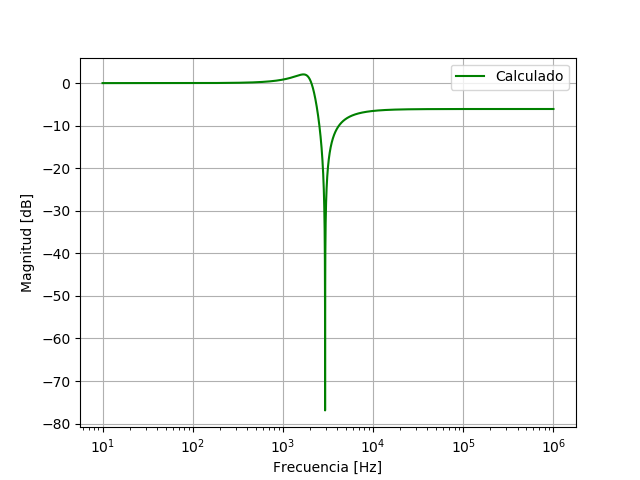
\includegraphics[width=1.3\textwidth]{Imagenes/bodemag_calc.png}
	\end{subfigure}
	\begin{subfigure}[t]{0.49\textwidth}
	\centering
		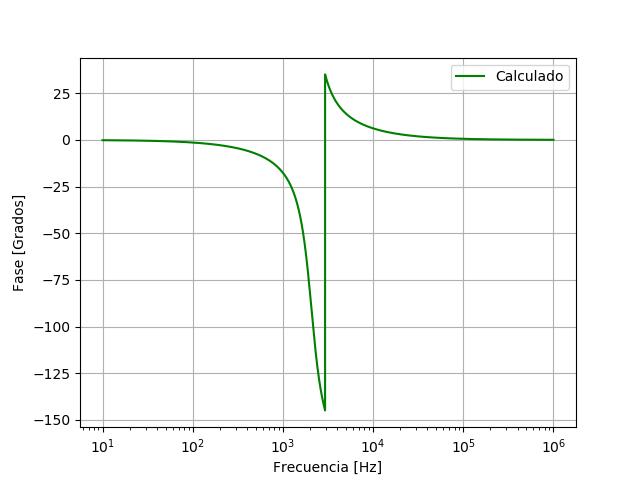
\includegraphics[width=1.3\textwidth]{Imagenes/bodefase_calc.png}
	\end{subfigure}
	\label{fig:bode_calc}
	\caption{Gráficos de Bode para el filtro con los componentes de valor comercial.}
\end{figure}

A continuación se presenta una tabla con los valores significantes de la respuesta en frecuencia.

\begin{table}[H]
\centering
\begin{tabular}{@{}ccccccc@{}}
\toprule
- & $\omega_z$ & $\omega_p$ & Q & $G_{Banda Pasante}$  & $G_{Notch}$ & $G_{Banda Atenuante}$ \\ \midrule
Valor deseado & $2926Hz$ & $2069Hz$ & $2$ & - & - & - \\
Valor calculado & $2930Hz$ & $2066,3Hz$ & $2.01$ & $0$ & $-76.91dB$ & $-6.08dB$ \\ 
Error & $0.135\%$ & $0.131\%$ & $0.546\%$ & - & - & - \\ \bottomrule
\end{tabular}
\caption{Valores significantes teóricos de la respuesta en frecuencia calculada.}
\label{tab:rta_freq_calc}
\end{table}

\subsubsection{Análisis de Ceros y Polos}

Se realizó un análisis de los ceros y polos de la transferencia ideal calculada tanto con los valores usados en la Tabla (\ref{Tab:valores}) como variando las resistencias $R_6$ y $R_8$.
A continuación se muestran los ceros y polos con los valores de la Tabla (\ref{Tab:valores}).

\begin{figure} [H]
	\centering
	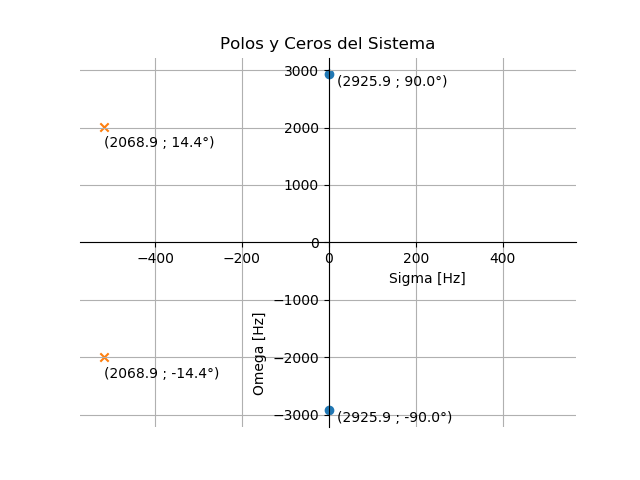
\includegraphics[width=0.8\textwidth]{Imagenes/cerosypolos_calc.PNG}
	\caption{Ceros y polos de la función transferencia ideal del circuito. Módulo y ángulo de cada cero y polo indicado.}
	\label{fig:cerosypolos_calc}
\end{figure}

Se puede observar como los polos y los ceros de la transferencia no se encuentran sobre una circunferencia de mismo radio, sino que los polos tienen una frecuencia de corte menor que la de los ceros. Esto genera que en el diagrama de Bode se encuentre primero el polo y luego el cero, por lo que la curva asintótica permanece por debajo de la línea del cero para las frecuencias mayores a la frecuencia de notch. Se puede contemplar además como los ceros se sitúan sobre el eje imaginario, por lo que el factor de calidad tiende a infinito y genera un gran sobrepico, atenuando casi totalmente las frecuencias cuyo valor sean igual al módulo de los ceros.

Luego, se procede a realizar un análisis del desplazamiento de los polos dadas variaciones en las resistencias $R_6$ y $R_8$. Cabe notar que el color más oscuro corresponde con la posición inicial de los ceros y polos.

\begin{figure}[H]
	\centering
	\begin{subfigure}[t]{0.49\textwidth}
	\hspace*{-2cm}
	\centering
		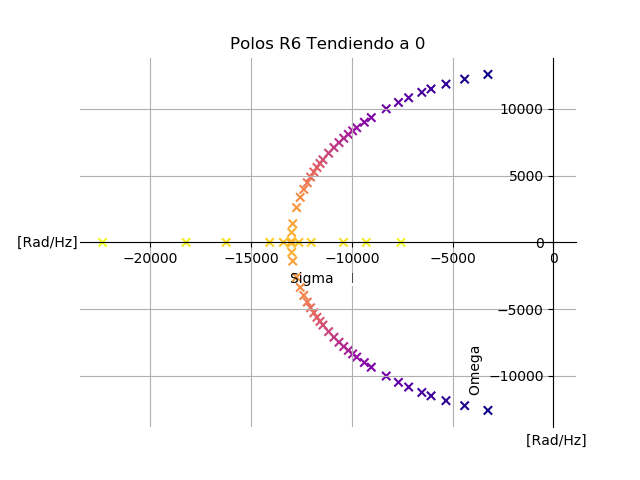
\includegraphics[width=1.2\textwidth]{Imagenes/polosr6a0.png}
	\end{subfigure}
	\begin{subfigure}[t]{0.49\textwidth}
	\centering
		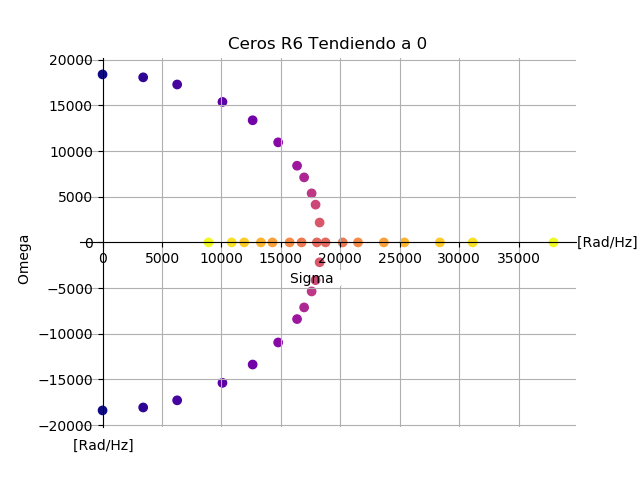
\includegraphics[width=1.2\textwidth]{Imagenes/cerosr6a0.png}
	\end{subfigure}
	\caption{Posición de los ceros y polos de la transferencia cuando $R_6$ parte de su valor original y tiende a cero.}
	\label{fig:r6a0}
\end{figure}

\begin{figure}[H]
	\centering
	\begin{subfigure}[t]{0.49\textwidth}
	\hspace*{-2cm}
	\centering
		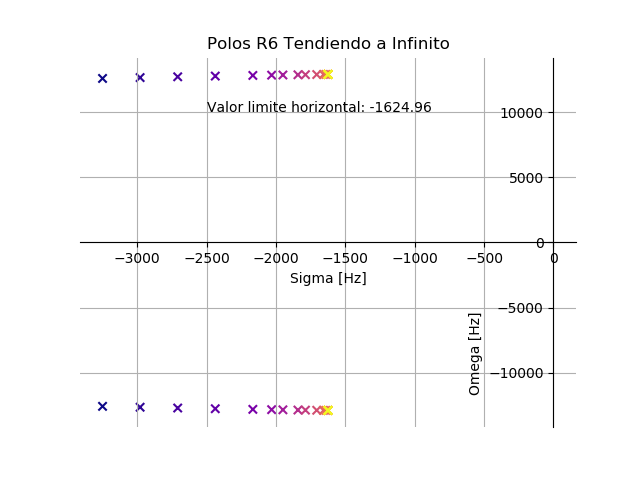
\includegraphics[width=1.2\textwidth]{Imagenes/polosr6ainf.png}
	\end{subfigure}
	\begin{subfigure}[t]{0.49\textwidth}
	\centering
		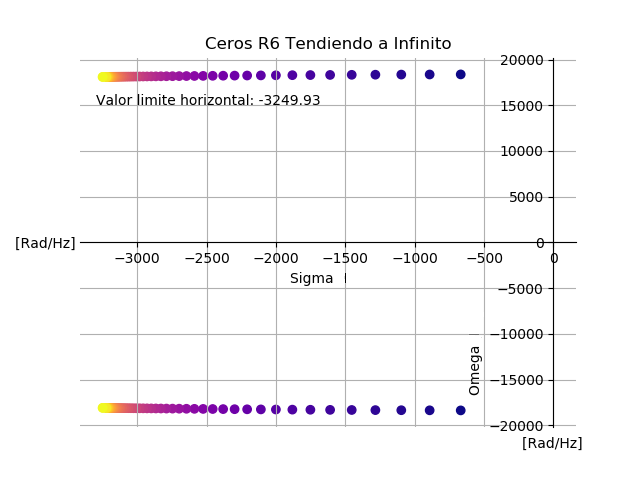
\includegraphics[width=1.2\textwidth]{Imagenes/cerosr6ainf.png}
	\end{subfigure}
	\caption{Posición de los ceros y polos de la transferencia cuando $R_6$ parte de su valor original y tiende a infinito.}
	\label{fig:r6ainf}
\end{figure}

Se puede observar en las Figuras (\ref{fig:r6a0}) y (\ref{fig:r6ainf}) que cambios en la resistencia $R_6$ genera que los ceros y polos no solo se desplacen horizontalmente sino también que estos transicionen de ser complejos conjugados, a estar ubicados en un mismo punto y eventualmente situarse solamente sobre el eje real, apartándose el uno del otro. Además, es observable como si $R_6$ aumenta de su valor original, disminuirá el sobrepico de los ceros y aumentará el sobrepico de los polos. Si $R_6$ tiende a cero, se contempla como baja el factor de calidad de tanto los ceros como los polos, por lo que el filtro pierde su naturaleza de notch y pasa a asemejarse más a la curva asintótica de la transferencia. Con este análisis se puede llegar a la conclusión que la resistencia $R_6$ regula el factor de calidad del circuito.


A continuación se analiza el desplazamiento de los polos variando la resistencia $R_8$. 

\begin{figure}[H]
	\centering
	\begin{subfigure}[t]{0.49\textwidth}
	\hspace*{-2cm}
	\centering
		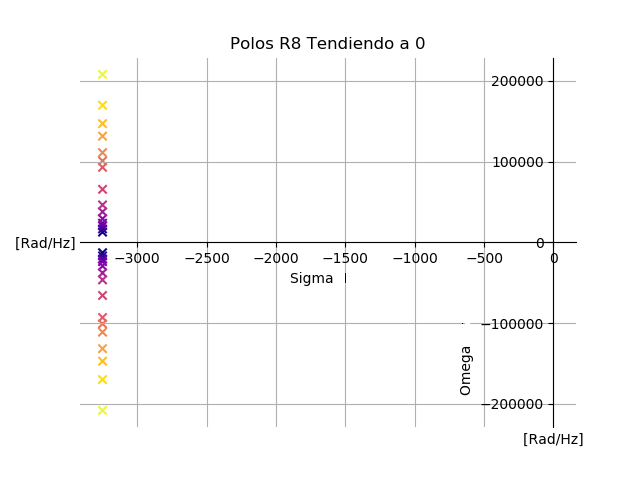
\includegraphics[width=1.2\textwidth]{Imagenes/polosr8a0.png}
	\end{subfigure}
	\begin{subfigure}[t]{0.49\textwidth}
	\centering
		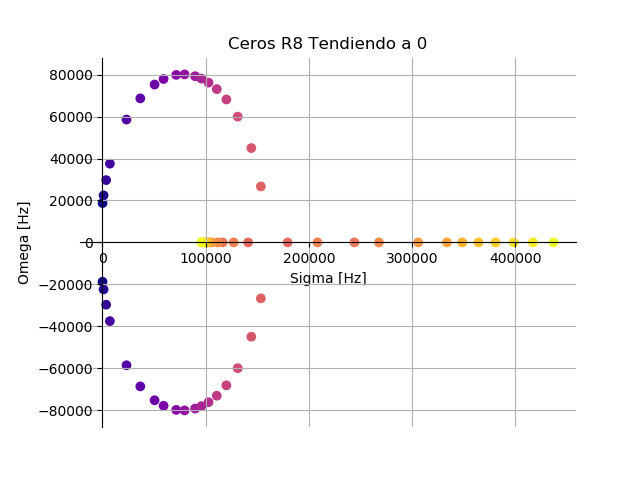
\includegraphics[width=1.2\textwidth]{Imagenes/cerosr8a0.png}
	\end{subfigure}
	\caption{Posición de los ceros y polos de la transferencia cuando $R_8$ parte de su valor original y tiende a cero.}
	\label{fig:r8a0}
\end{figure}

\begin{figure}[H]
	\centering
	\begin{subfigure}[t]{0.49\textwidth}
	\hspace*{-2cm}
	\centering
		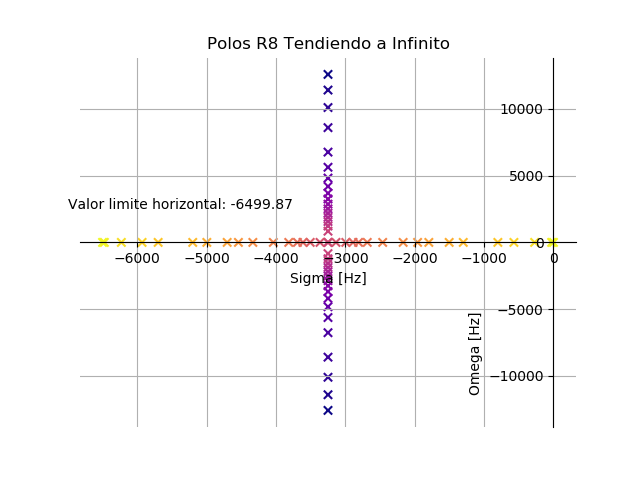
\includegraphics[width=1.2\textwidth]{Imagenes/polosr8ainf.png}
	\end{subfigure}
	\begin{subfigure}[t]{0.49\textwidth}
	\centering
		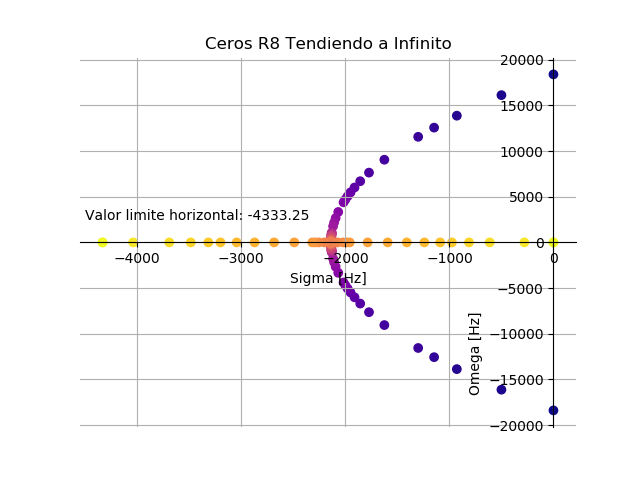
\includegraphics[width=1.2\textwidth]{Imagenes/cerosr8ainf.png}
	\end{subfigure}
	\caption{Posición de los ceros y polos de la transferencia cuando $R_8$ parte de su valor original y tiende a infinito.}
	\label{fig:r8ainf}
\end{figure}

Se contempla en las Figuras (\ref{fig:r8a0}) y (\ref{fig:r8ainf}) como pequeñas variaciones en la resistencia $R_8$ logra generar corrimientos en la frecuencia de notch del circuito, manteniendo aproximadamente su forma. Si las variaciones son muy extremas, se pierde la condición de notch ya que varía el factor de calidad del circuito.

Se puede concluir que la resistencia $R_8$ y sus pares regulan la frecuencia del notch, dentro de ciertos límites en los que la selectividad se conserva aproximadamente.

\subsubsection{Análisis de Sensibilidades}

El análisis de sensibilidades es una herramienta fundamental a la hora de diseñar no solo filtros, sino cualquier circuito electrónico. Este análisis permite conocer cuánto cambia un parámetro fundamental del circuito, como por ejemplo la selectividad, dada una variación en otro de sus parámetros, como por ejemplo una resistencia.

La sensibilidad de un parámetro $y$ respecto a otro parámetro $x$ se calcula como

\begin{equation}
S^y_x = \frac{x}{y} \frac{\partial y}{\partial x}
\end{equation}

Para el análisis de sensibilidades se remite a la función transferencia obtenida en la Sección (\ref{sec:fun_trans}) reescrita a continuación.

\[
\hspace{-0.5cm}
\frac{V_{out}}{V_i} = \frac{S^2 C_2 R_1 R_3 R_6 R_7 (-C_6 R_4 + C_7 R_8) + S C_2 R_1 R_3 (R_6 R_8 - R_4 R_7) + R_4 R_6 R_7}{S^2 C_2 R_1 R_3 R_6 R_7 R_8 (C_6 + C_7)+S C_2 R_1 R_3 R_8 (R_7 + R_6) + R_4 R_6 R_7}
\]

Como primer paso, se realiza un análisis de la sensibilidad de la frecuencia de notch $\omega_z$ en función de los componentes resistivos y capacitivos del circuito.

Considerando que
\begin{equation}
\omega_z = \frac{1}{\sqrt{C_2 R_1 R_3 R_6 R_7 (C_7 R_8 - C_6 R_4)}}
\end{equation}

se halla la derivada parcial de $\omega_z$ respecto de $R_1$ como

\begin{equation}
\frac{\partial \omega_z}{\partial R_1} = -\frac{1}{2} \frac{C_2 R_3 R_6 R_7 (C_7 R_8 - C_6 R_4)}{(C_2 R_1 R_3 R_6 R_7 (C_7 R_8 - C_6 R_4))^{\frac{3}{2}}}
\end{equation}

siendo finalmente la sensibilidad de la frecuencia de notch respecto de la resistencia $R_1$

\begin{equation}
S^{\omega_z}_{R_1} = - \frac{1}{2}  R_1 \sqrt{C_2 R_1 R_3 R_6 R_7 (C_7 R_8 - C_6 R_4)} \frac{C_2 R_3 R_6 R_7 (C_7 R_8 - C_6 R_4)}{(C_2 R_1 R_3 R_6 R_7 (C_7 R_8 - C_6 R_4))^{\frac{3}{2}}} = -\frac{1}{2}
\end{equation}

De forma análoga se calculó el resto de las sensibilidades de la frecuencia de notch respecto a los componentes resistivos y capacitivos presentados a continuación.

\begin{table}[H]
\centering
\begin{tabular}{@{}ccccccccc@{}}
\toprule
$S^{\omega_z}_{R_1}$ & $S^{\omega_z}_{C_2}$ & $S^{\omega_z}_{R_3}$ & $S^{\omega_z}_{R_4}$ & $S^{\omega_z}_{R_8}$ & $S^{\omega_z}_{R_6}$ & $S^{\omega_z}_{C_6}$ & $S^{\omega_z}_{R_7}$ & $S^{\omega_z}_{C_7}$  \\ \midrule
$-\frac{1}{2}$ & $-\frac{1}{2}$ & $-\frac{1}{2}$ & $\frac{1}{2}\frac{R_4 C_6}{C_7 R_8 - C_6 R_4}$ & $-\frac{1}{2}\frac{R_8 C_7}{C_7 R_8 - C_6 R_4}$ & $-\frac{1}{2}$ & $\frac{1}{2}\frac{R_4 C_6}{C_7 R_8 - C_6 R_4}$ & $-\frac{1}{2}$ & $-\frac{1}{2} \frac{R_8 C_7}{C_7 R_8 - C_6 R_4}$ \\ \bottomrule
\end{tabular}
\caption{Sensibilidades de la frecuencia de notch respecto a los componentes resistivos y capacitivos del circuito.}
\label{tab:sens_wz}
\end{table}

Dadas las sensibilidades obtenidas, se puede observar que solamente cuatro de aquellas son distintas de $\pm \frac{1}{2}$. Si no se tuviesen consideraciones para la implementaciones del circuito, se podría minimizar la sensibilidad de la frecuencia de notch respecto a los capacitores, ya que estos son los que tienen una mayor tolerancia. No obstante, utilizando las consideraciones de la implementación del circuito, sucede que las sensibilidades de $R_4$, $R_8$, $C_6$ y $C_7$ son iguales a $\frac{1}{4}(k^2-1)$ por lo que las sensibilidades respecto a estos componentes pueden llegar a tornarse muy alta cuanto más apartados estén los polos de los ceros en módulo. 

A continuación se presentan las sensibilidades de la frecuencia de corte de los polos en función de los componentes resistivos y capacitivos del circuito.

\begin{table}[H]
\centering
\begin{tabular}{@{}ccccccccc@{}}
\toprule
$S^{\omega_p}_{R_1}$ & $S^{\omega_p}_{C_2}$ & $S^{\omega_p}_{R_3}$ & $S^{\omega_p}_{R_4}$ & $S^{\omega_p}_{R_8}$ & $S^{\omega_p}_{R_6}$ & $S^{\omega_p}_{C_6}$ & $S^{\omega_p}_{R_7}$ & $S^{\omega_p}_{C_7}$  \\ \midrule
$-\frac{1}{2}$ & $-\frac{1}{2}$ & $-\frac{1}{2}$ & $0$ & $-\frac{1}{2}$ & $-\frac{1}{2}$ & $-\frac{1}{2}\frac{C_6}{C_6+C_7}$ & $-\frac{1}{2}$ & $-\frac{1}{2} \frac{C_7}{C_7+ C_6}$ \\ \bottomrule
\end{tabular}
\caption{Sensibilidades de la frecuencia de los polos respecto a los componentes resistivos y capacitivos del circuito.}
\label{tab:sens_wp}
\end{table}

Un resultado interesante es que variaciones en la resistencia $R_4$ no generan cambios en el posicionamiento de los polos, pero si generan cambios en el factor de calidad de ambas singularidades.

Otro resultado que destaca el análisis de las sensibilidades, tanto de los ceros como los polos, es como una variación en la resistencia $R_1$ de influye de misma manera en el posicionamiento de los polos y ceros por igual, por lo que se puede utilizar un preset en el lugar de esta resistencia para finamente calibrar la respuesta del circuito si esta se ve levemente corrida, sin perturbar la ganancia para las altas frecuencias.


El cálculo y la presentación de las sensibilidades de las selectividades de ambas singularidades se omitió por ser de carácter engorroso y resultar en la dependencia de muchos de los parámetros del circuito.

\subsubsection{Elección de los Amplificadores Operacionales}

Al momento de elegir el operacional a utilizar, se tuvo un claro objetivo: mantener las especificaciones del filtro fieles a lo calculado en el mayor rango de frecuencias posible. Es por esto que uno de los principales parámetros a estudiar en la selección del opamp fue el ancho de banda. Cuanto mayor sea este, más fidedigna será la transferencia en las altas frecuencias, ya que los polos del dispositivo estarán ubicados en mayores frecuencias cuanto más alto sea el ancho de banda.

Otro parámetro importante fueron aquellos que permiten lograr obtener una señal de salida con una baja distorsión armónica. En otras palabras, se buscó no deformar alinealmente a la señal de entrada introduciendo armónicos en esta. Para ello, se consideró la utilización de un amplificador operacional con un alto slew rate.

Finalmente se optó por utilizar el integrado TL-082 el cual posee dos amplificadores operacionales dentro. Se decidieron utilizar estos operacionales ya que poseen un slew rate alto ($13\frac{V}{\mu s}$ valor típico) en comparación a otros operacionales, un ancho de banda grande ($3MHz$ valor típico para ganancia unitaria) y además posee transistores de tecnología J-FET a la entrada del dispositivo, por lo que tanto la corriente de bias como la tensión de offset son más bajos que otro operacional con tecnología BJT a la entrada.

\subsection{Simulación del Circuito}
\label{sec:simulacion}

Se realizó la simulación del circuito utilizando el software \textit{LTSpiceXVII}.

\subsubsection{Simulación de la Transferencia}

Se procedió a realizar la simulación del circuito con los valores obtenidos mediante los paralelos en la Tabla (\ref{Tab:valores}). La primera simulación que se observó fue la respuesta en frecuencia.

\begin{figure}[H]
	\centering
	\begin{subfigure}[t]{0.49\textwidth}
	\hspace*{-2cm}
	\centering
		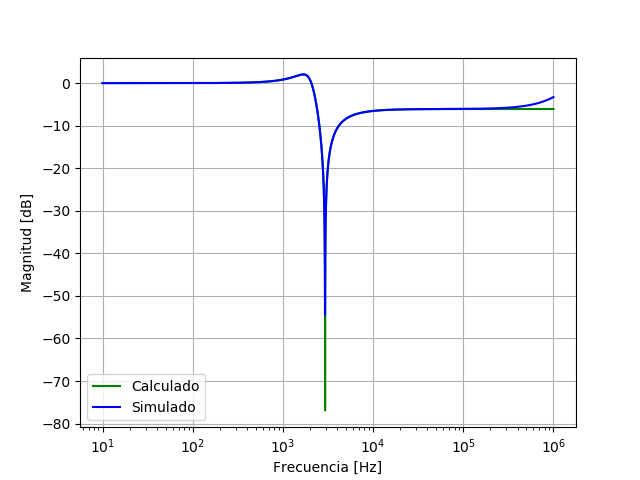
\includegraphics[width=1.3\textwidth]{Imagenes/bodemag_calc_sim.png}
	\end{subfigure}
	\begin{subfigure}[t]{0.49\textwidth}
	\centering
		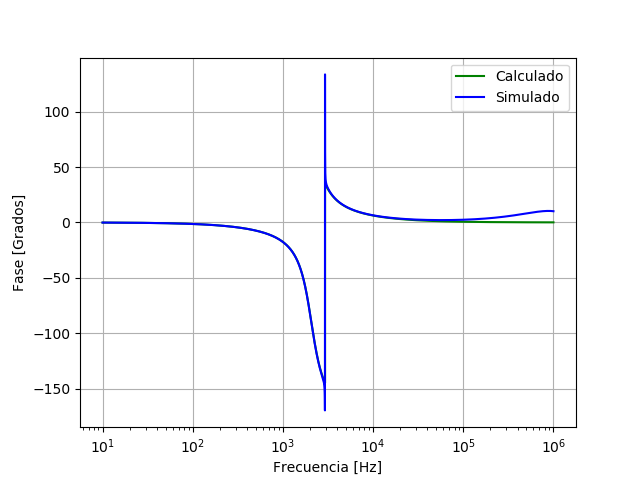
\includegraphics[width=1.3\textwidth]{Imagenes/bodefase_calc_sim.png}
	\end{subfigure}
	\caption{Comparación entre los gráficos de bode simulados y calculados teóricamente.}
	\label{fig:bode_calc_sim}
\end{figure}

Utilizando el operacional elegido en la sección \ref{sec:eleccion_componentes}, se observa una respuesta en frecuencia muy similar a la calculada anteriormente, exceptuando dos puntos de interes.

La ganancia en la frecuencia de notch es mucho menor a la calculada. Esto es algo esperado, ya que muchas cosas que no se tienen en consideración en los cálculos logran llegar a un resultado mucho más ideal que el real.

Respecto a las altas frecuencias, se puede observar una discrepancia entre lo calculado y lo teórico. Esta diferencia es mucho más grande tendiendo a las frecuencias cercanas a los $10MHz$. A continuación se grafica el Bode en fase y magnitud entre las frecuencias de los $100KHz$ y los $100MHz$.

\begin{figure}[H]
	\centering
	\begin{subfigure}[t]{0.49\textwidth}
	\hspace*{-2cm}
	\centering
		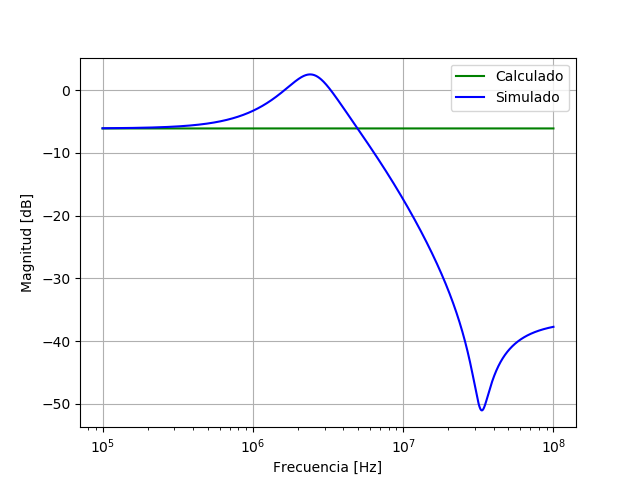
\includegraphics[width=1.3\textwidth]{Imagenes/bodemag_calc_sim_highf.png}
	\end{subfigure}
	\begin{subfigure}[t]{0.49\textwidth}
	\centering
		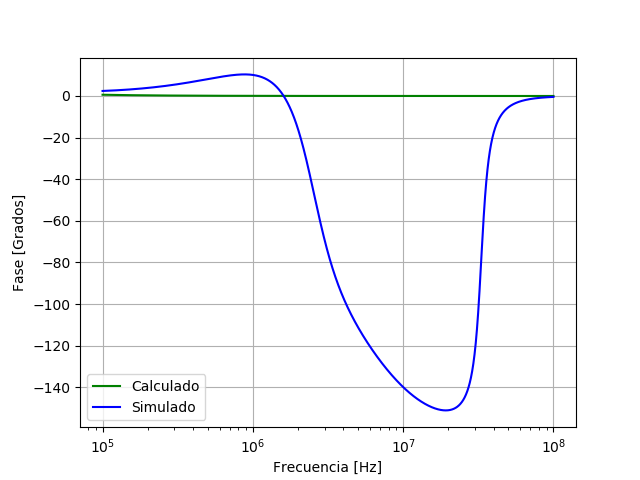
\includegraphics[width=1.3\textwidth]{Imagenes/bodefase_calc_sim_highf.png}
	\end{subfigure}
	\label{fig:bode_calc_sim_highf}
	\caption{Comparación entre los gráficos de bode simulados y calculados teóricamente para las frecuencias mayores a $100KHz$.}
\end{figure}

Si bien el operacional elegido posee un gran ancho de banda para mitigar lo más posible estos problemas a las altas frecuencias, como justificado en la Sección (\ref{sec:eleccion_componentes}), se puede observar que los cálculos realizados con el modelo ideal del operacional poseen una gran diferencia respecto a la simulación, la cual tiene en cuenta los varios polos que posee este dispositivo. Debido a esto, se tendrá en cuenta en la Sección (\ref{sec:limitaciones}) las limitaciones del filtro.

\subsubsection{Simulación de la Impedancia de Entrada y Salida}

Se observó luego la impedancia de entrada y salida del circuito.

\begin{figure}[H]
	\centering
	\begin{subfigure}[t]{0.49\textwidth}
	\hspace*{-2cm}
	\centering
		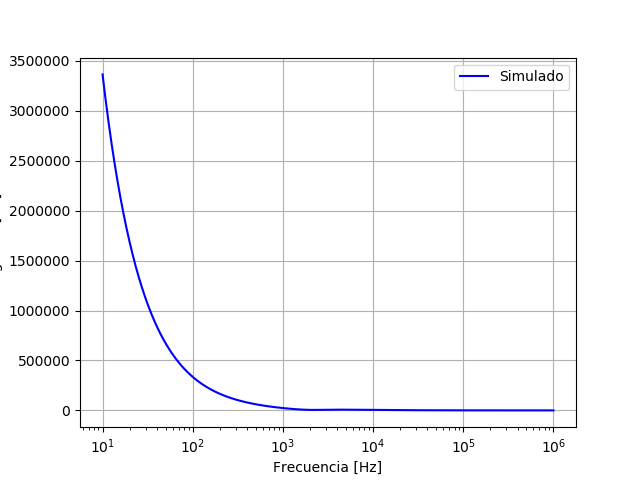
\includegraphics[width=1.3\textwidth]{Imagenes/sim_zin.png}
		\caption{Módulo de la impedancia de entrada.}
	\end{subfigure}
	\begin{subfigure}[t]{0.49\textwidth}
	\centering
		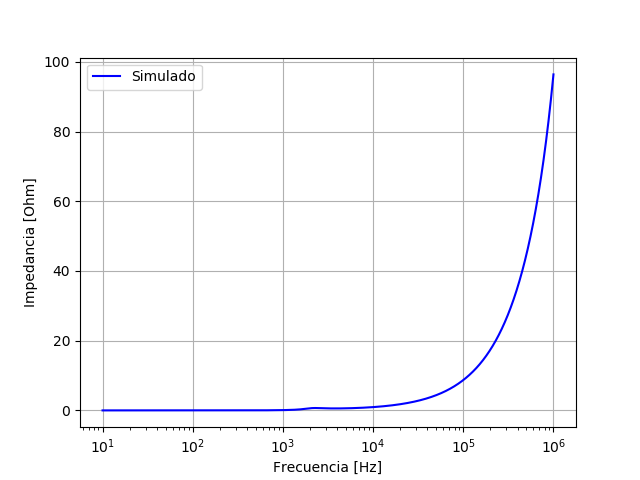
\includegraphics[width=1.3\textwidth]{Imagenes/sim_zout.png}
		\caption{Módulo de la impedancia de salida.}
	\end{subfigure}
	\label{fig:zin_zout}
	\caption{Simulación de la impedancia de entrada y salida del circuito.}
\end{figure}

Se puede ver como tanto la impedancia de entrada como de salida tienden a un valor nulo cuanto más alta la frecuencia. Esto era esperable ya que tanto a la entrada se encuentran dos capacitores cuyo camino a través de ellos lleva a tierra como a la salida se encuentra la impedancia de salida del operacional la cual es muy chica. Esto puede llegar a traer varios problemas a la hora de realizar las mediciones del filtro una vez implementado, por lo que se debe tomar un especial cuidado en esta etapa del análisis. 

\subsubsection{Simulación Montecarlo}
Se utilizó la simulación Montecarlo para observar la dispersión de la respuesta en frecuencia causada por las tolerancias de los componentes. Se utilizó una tolerancia del 5\% para todos los resistores excepto 1\% para las resistencias de 9k1. Para los capacitores se utilizó una tolerancia del 10\%.

\begin{figure}[H]
	\centering
	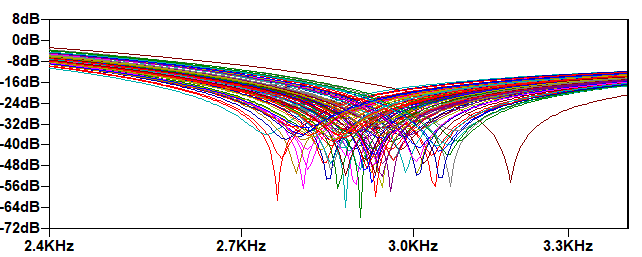
\includegraphics[width=\textwidth]{Imagenes/Montecarlo1.PNG}
	\caption{Simulación de Montecarlo.}
	\label{fig:montecarlo}
\end{figure}

Se puede observar una gran dispersión en la frecuencia de notch de aproximadamente $300Hz$ sin tomar en cuenta el caso de más a la derecha.

\subsection{Implementación del Circuito}
Se implementó el circuito siguiendo las consideraciones y el análisis realizado en la Sección (\ref{sec:eleccion_componentes}). Se decidió utilizar una placa 5x5, resistores al 1\% y 5\% y capacitores de film al 10\%. También se optó por utilizar dos capacitores de desacople de tecnología SMD con un valor de $100nF$ colocados lo más próximo al operacional como posible. 
\subsubsection{Mediciones del Circuito y Análisis de Error}
\subsubsection{Limitaciones del Circuito}
\label{sec:limitaciones}

\begin{center}
	\textcolor{\textbf{slewrate+saturacion ver entrada maxima.}}\\
	\textcolor{\textbf{ver alimentacion minima por saturacion y entrada maxima.}}\\
	\textcolor{\textbf{ver conjunto de frecuencias donde se puede usar piola.}}\\
\end{centerc


Se ha recopilado, de la hoja de datos del \hypref{http://www.ti.com/lit/ds/symlink/tl082.pdf}{TL-082}, los parámetros utilizados en el análisis de las limitacionnes del circuito.

\begin{table}[H]
\centering
\begin{tabular}{@{}ccccc@{}}
\toprule
$V_{CC_{max}}$ & $V_{in_{max}}$ & $BW_{unitgain}$ & $V_{in_{max}}$ dada $V_{CC}$ & Slew Rate (SR)\\ \midrule
$\pm 18V$ & $\pm 15V$ & $3MHz$ & $\approx V_{CC}-1.5V$ & $13\frac{V}{\mu s}$\\ \bottomrule
\end{tabular}
\caption{Datos recopilados de la hoja de datos del TL-082.}
\label{tab:datos_tl082}
\end{table}

Observando la tabla se puede corroborar que la tensión de alimentación no debe sobrepasar los $18V$, mientras que la de entrada no debe sobrepasar los $15V$. Para el análisis de las limitaciones del circuito, sin embargo, se utilizarán $\pm 15V$ de alimentación, valor recomendado por el fabricante.
Luego, teniendo en cuenta que la ganancia máxima del circuito es de $\approx 2dB$, se tiene que

\begin{equation}
	V_{in_{max}} = \frac{V_{CC} - 1.5V}{G_{max}} = \frac{13.5V}{1.26} = 10.72V
\end{equation}

Sin embargo, también se debe de tener en cuenta el slew rate en el análisis de la tensión de entrada máxima.

\begin{equation}
	SR= Max\left( \frac{\partial (G\cdot A\cdot \sin (\omega t))}{\partial t}\right) = V_{in} \cdot \omega \cdot G  
\end{equation}

Primero se analiza la tensión máxima de entrada en la frecuencia de sobrepico ya que esta posee la ganancia más alta.

\begin{equation}
	V_{in_{max}} = \frac{SR}{G_{max}\cdot \omega} = \frac{1.64\cdot 10^6\frac{V}{s}}{1686Hz} = 972.71
\end{equation}

Luego se analiza la tensión máxima de entrada para las frecuencias altas.

\begin{equation}
	V_{in_{max}} = \frac{SR}{G_{Banda Atenuante}\cdot \omega} = \frac{2.01\cdot 10^6\frac{V}{s}}{f}
\end{equation}

Por lo que se graficó la tensión máxima de entrada final en función de la frecuencia tomando en consideración los cálculos previos.

\begin{figure} [H]
	\centering
	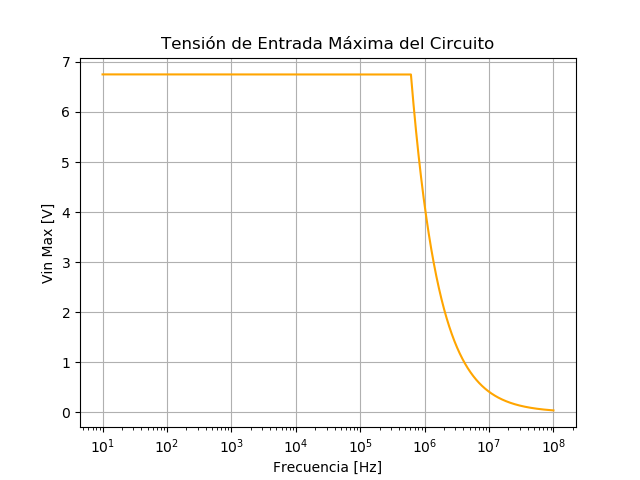
\includegraphics[width=0.7\textwidth]{Imagenes/vin_max.PNG}
	\caption{Tensión de entrada máxima del circuito en función de la frecuencia teniendo en cuenta distorsiones alineales causadas por el operacional.}
	\label{fig:vin_max}
\end{figure}

Luego, el rango de frecuencias en que el circuito opera correctamente, dato conseguido empíricamente, es hasta 1Mhz.


\subsection{Conclusiones}

\subsection{Bibliografía Utilizada}
[1]F. Sergio, Design with operational amplifiers and analog integrated circuits, 4th ed. New York [etc.]: McGraw-Hill, 1988, p. 185.

[2]F. Sergio, Design with operational amplifiers and analog integrated circuits, 4th ed. New York [etc.]: McGraw-Hill, 1988, p. 186.

[3]F. Sergio, Design with operational amplifiers and analog integrated circuits, 4th ed. New York [etc.]: McGraw-Hill, 1988, p. 187.


\end{document}